\documentclass{standalone}

\usepackage{luatex85}
\usepackage{tikz}
\usetikzlibrary{calc}

\begin{document}
    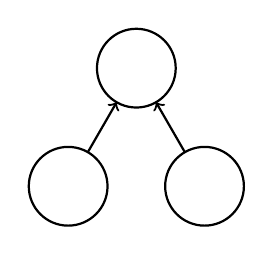
\begin{tikzpicture}
        \pgfmathsetmacro{\sepRadius}{1}
        \pgfmathsetmacro{\sphereRadius}{0.5}
        \foreach \i in {0,...,2}{
            \draw[thick] (90 + deg{2*pi*\i/3}: \sepRadius) circle(\sphereRadius);
        }
        \foreach \i in {-1, 1}{
            \draw[->, thick]
                ($(90 + \i*deg{2*pi/3}: \sepRadius) + (90 - \i*deg{pi}/6: \sphereRadius)$) --
                ($(90: \sepRadius) + (-90 - \i*deg{pi/6}: \sphereRadius)$);
        }
    \end{tikzpicture}
\end{document}
